\documentclass[11pt]{article}

\usepackage{graphicx}
\graphicspath{ {./Imagenes/} }

% Margins
\topmargin=-0.45in
\evensidemargin=0in
\oddsidemargin=0in
\textwidth=6.5in
\textheight=9.0in
\headsep=0.25in

\title{ REASONING AGENTS }
\author{ Govardhan Chitrada }
\date{\today}

\begin{document}
\maketitle	
\pagebreak

% Optional TOC
% \tableofcontents
% \pagebreak

%--Paper--

\section{Reinforcement Learning}

% Bold in latex is \textbf{}

\textbf{Reinforcement Learning} is a type of machine learning that uses a reward function to guide the agent in deciding which action to take. The agent is rewarded for taking the action that maximizes the reward function.
In general, a Reinforcement learning agent is able to perceive and interpret the environment and learn from it. By adding a method of rewarding desired behaviors and punishing undesired behaviors. This programs the agent to 
seek long term and maximum overall reward to achieve an optimal solution.

% Write working of reinforcement learning in 100 lines as latex format
While reinforcement learning has been a topic of much interest in the field of AI, its widespread, real-world adoption and application remain limited. Noting this, however, research papers abound on theoretical applications, 
and there have been some successful use cases.

Current use cases include, but are not limited to, the following:
\begin{itemize}
    \item Reinforcement learning for autonomous driving
    \item  Reinforcement learning for autonomous navigation
    \item  Reinforcement learning for autonomous speech recognition
    \item Reinforcement learning for robotic manipulation
\end{itemize}
\subsection{Deep Reinforcement Learning}
Deep Learning uses artificial neural networks to map inputs to outputs. Deep Learning is powerful, because it can approximate any function with only one hidden layer¹. 
How does it work? The network exists of layers with nodes. The first layer is the input layer. Then the hidden layers transform the data with weights and activation functions. The last layer is the output layer, where the target is predicted. 
By adjusting the weights the network can learn patterns and improve its predictions.
As the name suggests, Deep Reinforcement Learning is a combination of Deep Learning and Reinforcement Learning. By using the states as the input, values for actions as the output and the rewards for adjusting the weights in the right direction, 
the agent learns to predict the best action for a given state.
\begin{figure}[h]
    \centering
    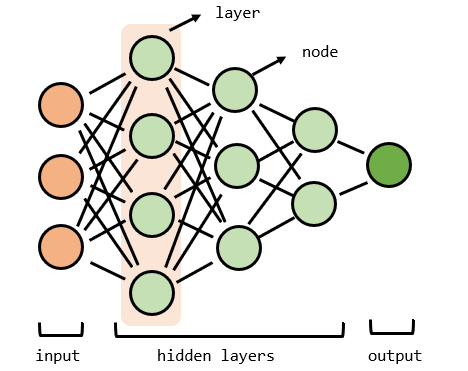
\includegraphics[width=0.25\textwidth]{neural-net}
    \caption{Simple neural network}
    \label{fig:neural_net}
\end{figure}


\pagebreak
\subsection{Deep Q Network - DQN}
Reinforcement learning can be sufficiently applicable to the environment where the all achievable states can be manged (iterated) and stored in standard computer RAM memory. However, the environment where the number of states overwhelms the 
capacity of contemporary computers (for Atari games there are 12833600 states) the standard Reinforcement Learning approach is not very applicable. Furthermore, in real environment, the Agent has to face with continuous states (not discrete), continuous variables and continuous control (action) problems.

Bearing in mind the complexity of environment the Agent has to operate in (number of states, continuous control) the standard well defined Reinforcement Learning Q — table is replaced by Deep Neural Network (Q — Network) which maps (non — linear approximation) environment states to Agent actions. Network architecture, choice of network hyper parameters and learning is performed during training phase (learning of Q — Network weight).
DQN allows the Agent to explore unstructured environment and acquire knowledge which over time makes them possible for imitating human behavior.
\subsection{DQN - Algorithm}

\begin{figure}[h]
    \centering
    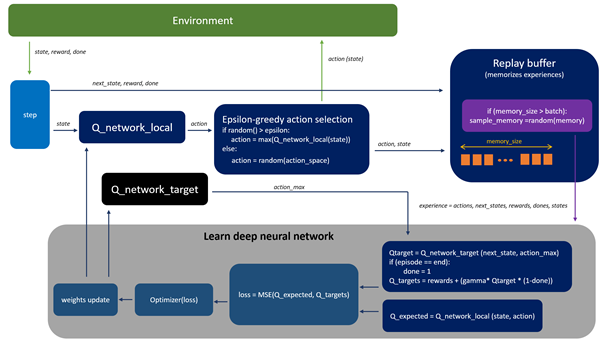
\includegraphics[width=1.0\textwidth]{dqn}
    \caption{DQN Algortihm}
    \label{fig:dqn}
\end{figure}

The above Fig \ref{fig:dqn} shows the DQN algorithm during the training process. 
where Q — network proceeds as a as nonlinear approximation which maps both state into an action value.
During the training process, the Agent, interacts with the environment and receives data, which is used during the learning the Q — network. The Agent explores the environment to build a complete picture of transitions and action outcomes. At the beginning the Agent decides about the actions randomly which over time becomes insufficient. While exploring the environment the Agent tries to look on Q — network (approximation) in order to decide how to act. 
We called this approach (combination of random behavior and according to Q — network) as an epsilon — greedy method (Epsilon -greedy action selection block), which just means changing between random and Q policy using the probability hyper parameter epsilon.

The core of presented Q-learning algorithm is derived from the supervised learning.
Here as it was mention above, the goal is to approximate a complex, nonlinear function Q(S, A) with a deep neural network.

During the process we use two seperate networks Q — network and target Q — network. The Q — network is used to approximate the Q function. The target Q — network is used to approximate the target Q function.
The target network is frozen for several time steps and then the target network weights are updated by copying the weights from the actual Q network. 
Freezing the target Q — network for a while and then updating its weights with the actual Q network weights stabilizes the training.


In short the algorithm can be described as follows:
\begin{enumerate}
    \item Initialize the Q — network with random weights.
    \item Initialize replay buffer
    \item Pre-process the environment and store the initial state in the replay buffer.
    \item Initialize the target Q — network with random weights.
    \item  For each episode:
        \begin{enumerate}
            \item Choose an action at random.
            \item Take action and observe the reward and the next state.
            \item Store the transition in the replay buffer.
            \item Sample a random minibatch from the replay buffer.
            \item Update the weights of the Q — network using the minibatch.
            \item Update the weights of the target Q — network using the minibatch.
        \end{enumerate}
    \item After the training is finished, the target Q — network weights are copied to the Q — network weights.
\end{enumerate}
\subsection{DQN Agent}

The methods \textit{reset(self),} \textit{step(self,action),} and \textit{get\_state(self).}. It is also necessary to calculate the reward every time the agent takes a step.
\begin{table}[ht]
\begin{center}
\begin{tabular}{ | c | c| }
\hline
 Param name & optimized values \\ 
\hline
\textit{epsilon}  & 1 \\  
\textit{epsilon\_min} & 0.01  \\ 
\textit{gamma} & 0.95 \\
\textit{batch\_size} & 500 \\
\textit{learning\_rate} & 0.00025 \\
\textit{layer\_sizes} & [128,128,128] \\
\hline
\end{tabular}
\label{tab:parameter-table}
\caption{Optimized Hyper-parameters for \textbf{DQN}.}
\end{center}

\end{table}

The agent learns to play snake (with expreience replay) and to avoid the obstacles. The following four state spaces are used:
\begin{itemize}
    \item \textit{observation} - the state of the environment.
    \item \textit{action} - the action taken by the agent.
    \item \textit{reward} - the reward received by the agent.
    \item \textit{next\_observation} - the next state of the environment.
\end{itemize}
\section{Environment - Snake}
In this specific project the game "Snake" is modified to fit certain requirements. The game is played on a grid of size 20x20. 
The snake is controlled by the agent. The agent is rewarded for eating food and for avoiding the walls and itself. 
The agent is penalized for running into itself. To this we also added two different food types such as meat and apple. In general,
to stay healthy in real life people should balance their diet with fruits and meat. In the same way here the snake has to eat maximum amount of food and
in the same way it has to alternate the food (We call it as pairs).

The rewards for eating the food are assigned by the Reinforcement learning agent  and the rewards for eating the food in alternative are assigned by the reasoning agent. 
The reasoning agent is a simple agent which tries to find the optimal solution for the agent.
\begin{figure}[h]
    \centering
    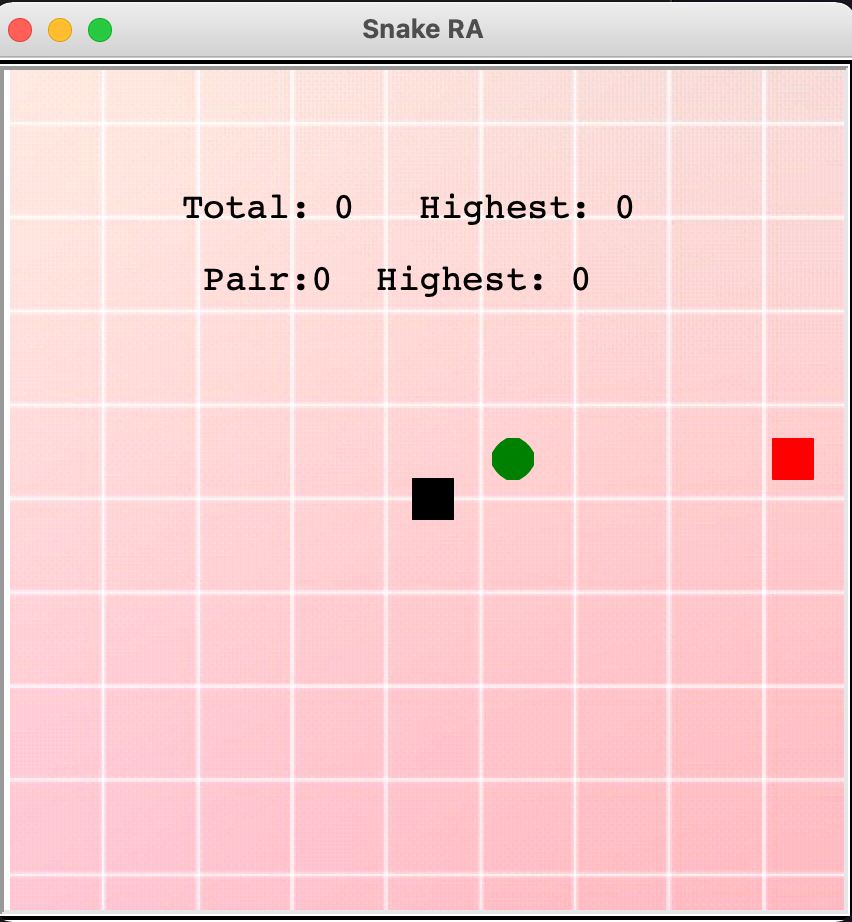
\includegraphics[width=0.5\textwidth]{env}
    \caption{Snake Environment}
    \label{fig:snake_env}
\end{figure}

In the above Fig.\ref{fig:snake_env} the environment is represented. The snake is represented by a black square. The food is represented by a green circle (apple) and red square (meat).
%--/Paper--
\subsection{Actions, rewards and states}
The agent can choose between going up, right, down or left. The rewards and state space are a bit harder. There are multiple solutions, and one will work better than the other. For now, let’s try the following. If the snake grabs an apple, give a reward of 10. If the snake dies, the reward is -100. To help the agent, give a reward of 1 if the snake comes closer to the apple, 
and a reward of -1 if the snake moves away from the apple. And coming to the state, where scaled coordinates of the snake and apple are the same, the state is 1. Adding the location of obstacles so the agent learns to avoid them.
Here is the set of \textbf{actions}:
\begin{itemize}
    \item \textit{UP} - the snake moves up.
    \item \textit{RIGHT} - the snake moves right.
    \item \textit{DOWN} - the snake moves down.
    \item \textit{LEFT} - the snake moves left.
\end{itemize}
The tables below show the state space and the reward space. These are the same for the agent and the reasoning agent.
% Create table with two columns and four rows

\begin{table}[ht]
\begin{center}
\begin{tabular}{ |c | c| }
\hline
 For eating an apple  & 10 \\ 
\hline
 For coming closer to apple  & 1 \\  
\hline
 For going away from apple & -1  \\ 
\hline
 For hitting the wall or itself & -100  \\ 
\hline
\end{tabular}
\end{center}
\label{tab:rewards-table}
\caption{Set of \textit{rewards}.}
\end{table}

\begin{table}[ht]
\begin{center}
\begin{tabular}{ |c | c| }
\hline
 Food above the snake & 0/1  \\
\hline
    Food below the snake  & 0/1 \\
\hline
Food on right side of the snake & 0/1  \\
\hline
    Food on left side of the snake  & 0/1 \\
\hline
Wall above the snake & 0/1  \\
\hline
    Wall on the right  & 0/1 \\
\hline
Wall below the snake & 0/1  \\
\hline
    Wall on the left  & 0/1 \\
\hline
Snake direction is up & 0/1  \\
\hline
    Snake direction is down  & 0/1 \\
\hline
Snake direction is left & 0/1  \\
\hline
    Snake direction is right  & 0/1 \\
\hline
\end{tabular}
\end{center}
\label{tab:state-table}
\caption{Set of \textit{states}.}
\end{table}
Tab \ref{tab:rewards-table} and \ref{tab:state-table} are used to show the set of rewards and states of the environment.
\pagebreak
\section{Results}
From Fig.\ref{fig:results} Training the agent with the reasoning agent for 130 episodes with 10000 steps per episode. Approximately at 60 episodes the agent achieved a maximum reward
and the learning curve shows that the agent is learning rapidly in first fifty episodes.
\begin{figure}[h]
    \centering
    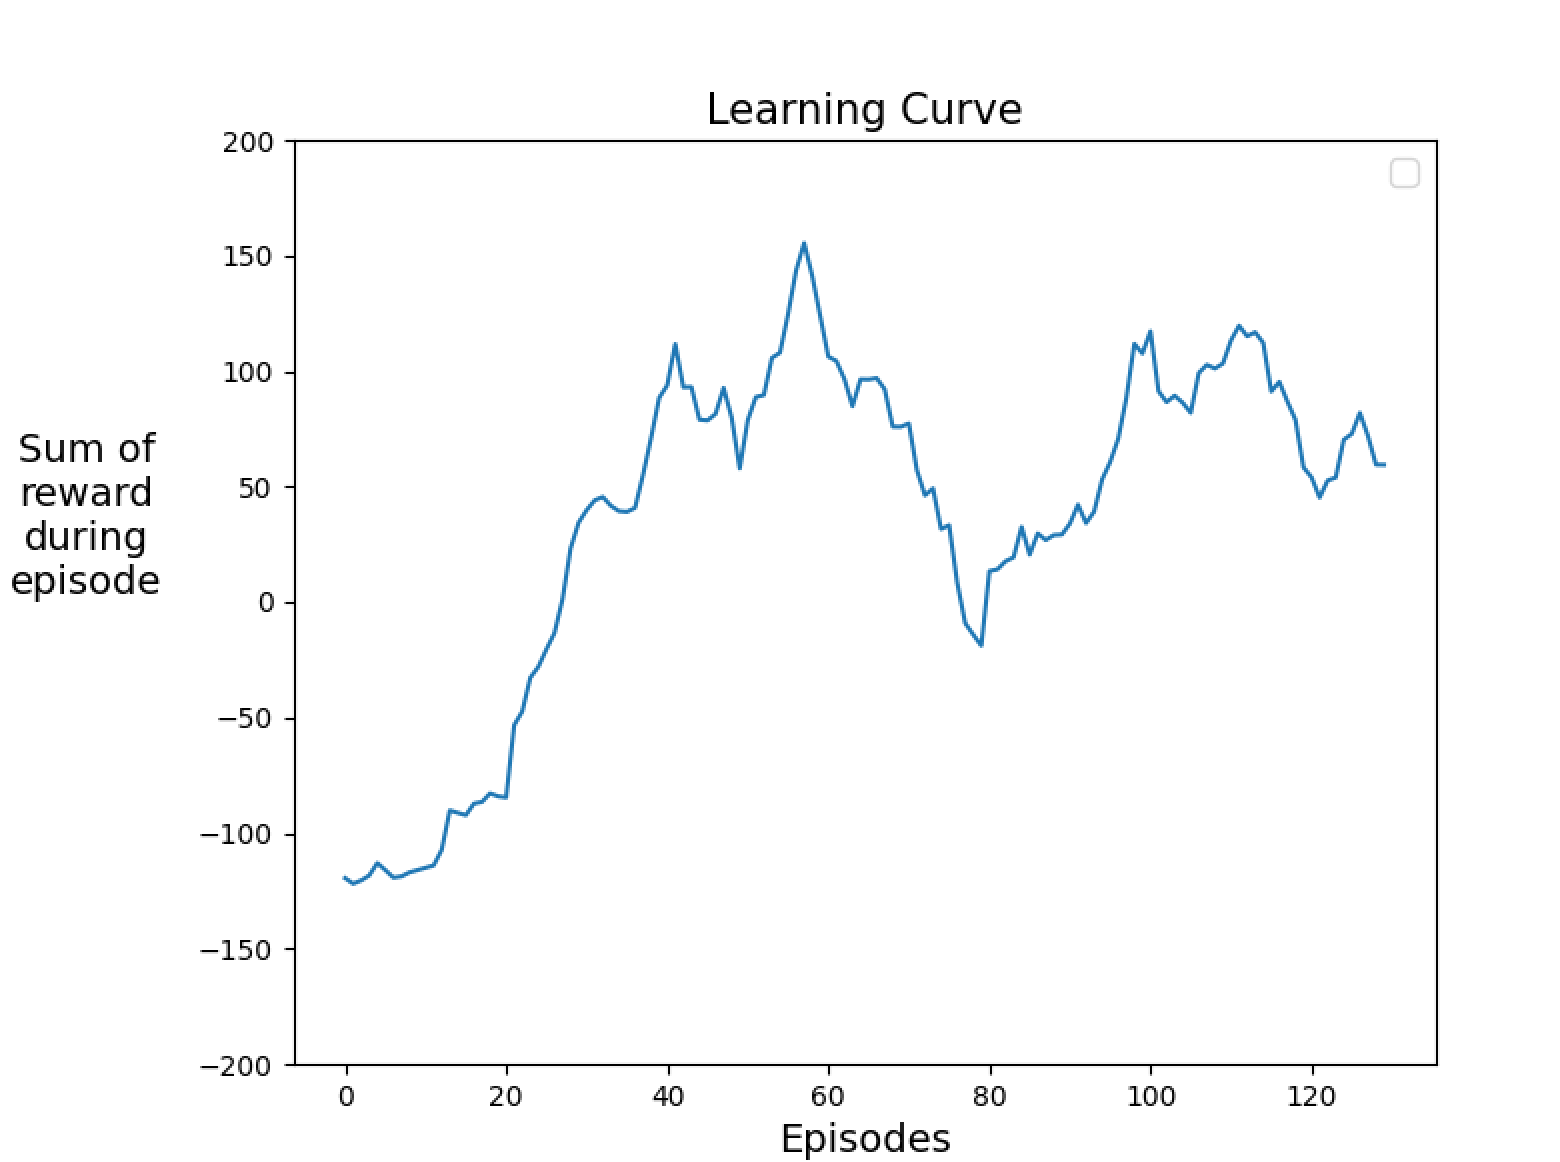
\includegraphics[width=0.5\textwidth]{graph2}
    \caption{Represents the \textbf{learning curve} and the maximum \textbf{reward}.}
    \label{fig:results}
\end{figure}
\begin{figure}[h]
    \centering
    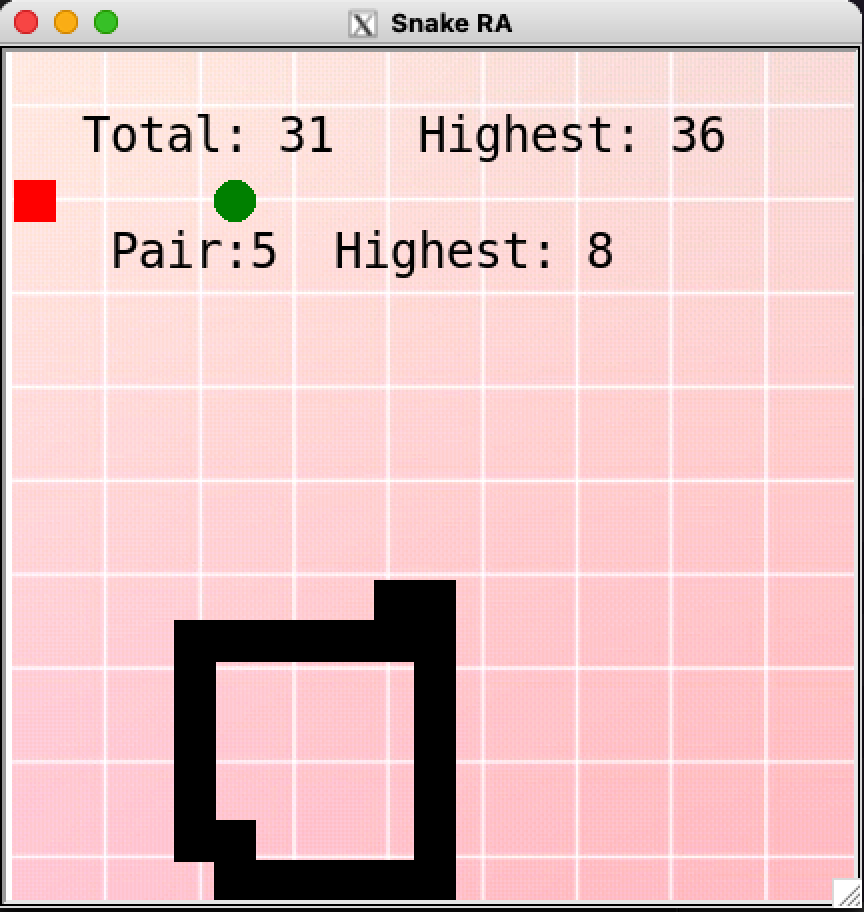
\includegraphics[width=0.5\textwidth]{trained-snake}
    \caption{The snake represents the trained \textbf{agent}.}
    \label{fig:trained-snake}
\end{figure}

From Fig.\ref{fig:trained-snake} we can say that the agent has learned to eat the food in way which avoids the wall and hitting itself.
Then the reward is given to the DQN agent and in the sameway the reasoning agent is rewarded when the snake eats food in pairs(red, green)
As we can see in the figure the agent is able to achive a pair score of 8 and total food score of 36 which is really good.
\end{document}
